\section{Ambiente e salute}

CRONACA: 2 morti di meningite all'Università Statale di Milano.

Nel primo dei 2 casi è stato fatto l'isolamento, si trattava di
meningococco C (il secondo caso è in accertamento).

La meningite è una malattia ad eziologia batterica o virale. Può essere
una malattia molto grave, ma è a bassa contagiosità! Essendo la
meningite una malattia che si trasmette per via aerea, le comunità
chiuse sono più a rischio ma la contagiosità è bassa.

Quando si è di fronte a casi gravi, si pone il problema della profilassi
dei contatti. La vaccinazione anti-meningococco non serve a nulla in un
caso di emergenza come questo: se si hanno contatti stretti si prescrive
la profilassi antibiotica. La vaccinazione non ha molto senso, perché
protegge la gittata più lunga, e non ha neanche senso intervenire con
delle vaccinazioni in una città piuttosto che in un'altra (è la logica
emozionale che porta a dire `facciamo il vaccino a tutti le persone
dell'Università di Milano'). Quindi, nei casi di contatti stretti è
giustificata una profilassi antibiotica, per il resto si continua con la
logica di una profilassi generale che vuole arrivare a proteggere tutti
i nuovi nati e con ciò ridurre la circolazione dei meningococchi al
fine, nel tempo, di ridurre i casi di meningite nelle categorie che non
sono state vaccinate.

Per certe categorie, come personale sanitario, può essere giustificata
una vaccinazione in età adulta però il normale approccio è fare le
vaccinazioni all'età in cui sono consigliate (1\textsuperscript{o} anno di vita per
anti-meningococco B e 2\textsuperscript{o}anno di vita per vaccino bivalente A C o
quadrivalente A C Y W135).

\subsection{Politiche ambientali in relazione alla salute umana}

EUROBAROMETRO 2011: 90\% dei cittadini europei intervistati si dichiara
preoccupato per l'ambiente.

Quali sono i motivi della preoccupazione?

\begin{itemize}
\item
  40\% disastri causati dall'uomo
\item
  36\% inquinamento delle acque
\item
  32\% impatto dei rifiuti
\item
  30\% smog e mancanza di verde
\item
  distruzione delle risorse naturali
\item
  consumismo fine a se stesso
\item
  cambiamenti climatici
\end{itemize}

Riguardo le politiche ambientali, alcune hanno ancora problemi da
risolvere, altre hanno più paure che non effetti provati.

Es: radiazioni non ionizzanti, come ponti radio, telefonini, uv. Qualche
effetto c'è, ad esempio alcuni tumori cutanei riconoscono come fattori
di rischio l'esposizione ai raggi solari con altre concause. La paura,
che alcuni paventano, delle radiazioni non ionizzanti è infinitesimale
in confronto a quella di altri fattori di rischio. L'ambiente
tipicamente porta a delle percezioni dei rischi non necessariamente
legate ai rischi reali, questo è uno dei problemi presenti nelle
politiche ambientali.

Nel caso dell'ambiente, ci sono situazioni di percezione dei rischi
superiori ai rischi provati e si ha anche il contrario, cioè rischi
reali assolutamente trascurati.

Es: rischio radon. Il radon è un gas naturale, cancerogeno, che ci
troviamo in casa senza saperlo, laddove è presente nel terreno il
componente primario, l'uranio, che attraverso i pori del terreno e
attraverso le fondamenta penetra nelle case. È un rischio reale
largamente trascurato. Nessuno quando compra casa si pone il problema
del radon.

Tutte le politiche ambientali sono basate su alcune situazioni provate,
altre situazioni probabili.

Definizione: l'\textbf{AMBIENTE}, secondo l'OMS, può essere definito
come un \emph{sistema integrato di fattori antropici e fisici che
esercitano un effetto significativo ed apprezzabile sulla salute della
collettività}.

Si ritiene che 1/3 delle patologie, direttamente o indirettamente,
riconosca dei fattori ambientali come fattori di rischio primari e
secondari (compreso il clima tropicale per la trasmissione di malattie
infettive).

\begin{figure}[!ht]
\centering
	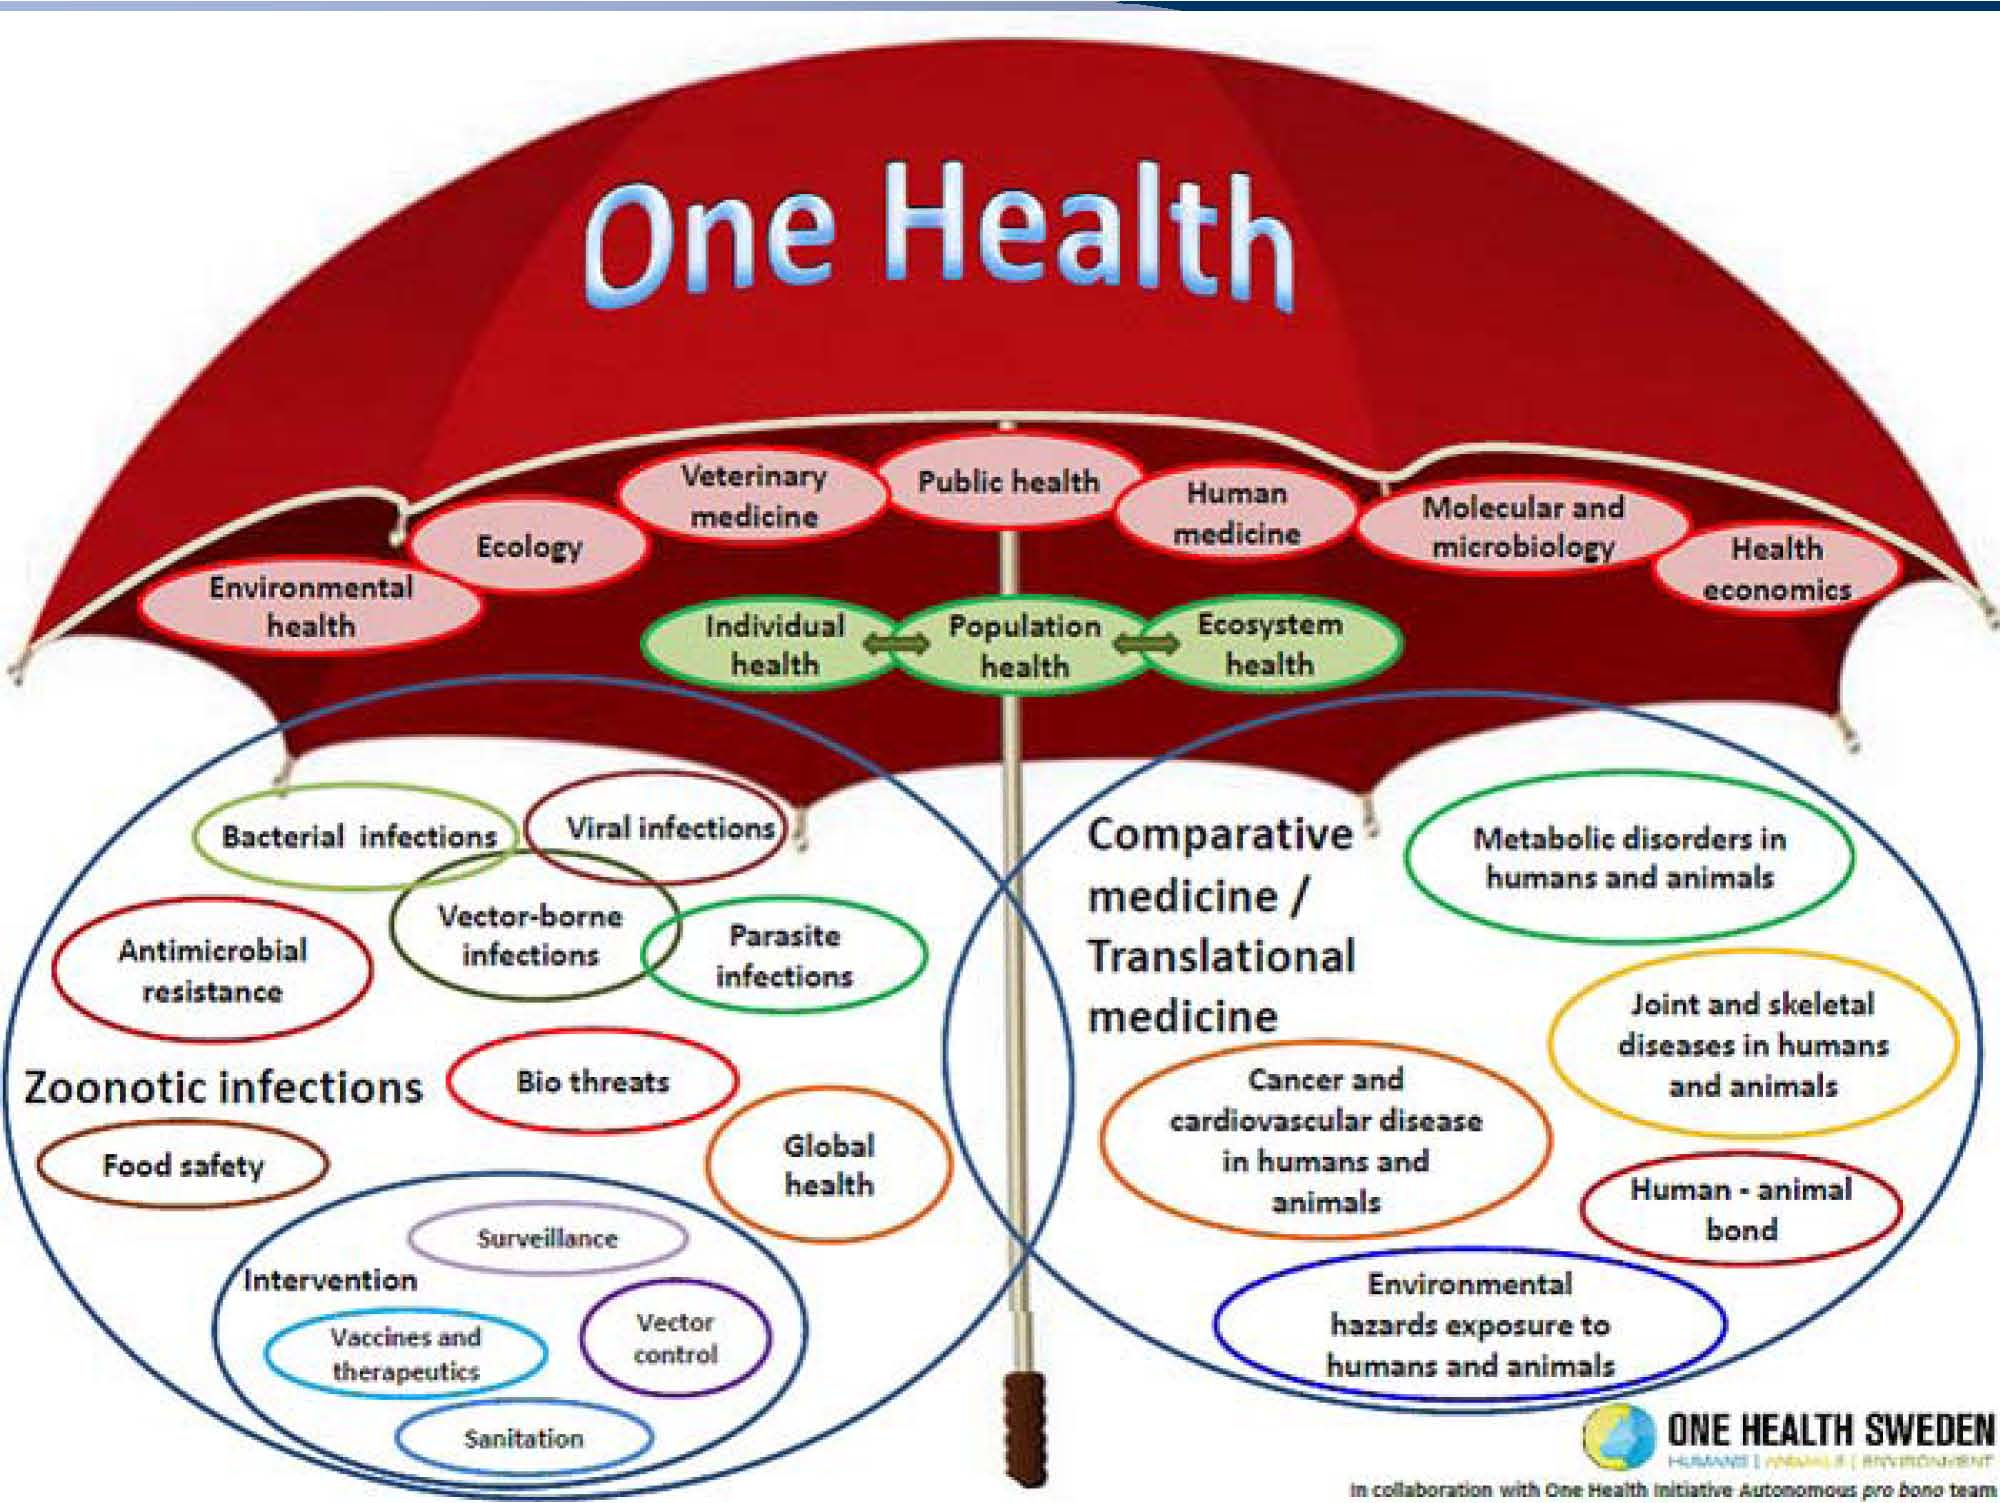
\includegraphics[width=0.7\textwidth]{22/image1.jpeg}
	\end{figure}

Importante notare come vi sia una stretta correlazione tra il mondo
fisico, l'ambiente, gli animali (alimenti di origine animale che possono
subire delle contaminazioni legate all'ambiente come acqua, suolo, cibo)
e salute umana.

Caso emblematico: mozzarelle con la diossina, derivate da discariche
abusive e non controllate in alcune province d'Italia, bestiame lasciato
liberamente nei campi utilizzati in passato come discarica conseguente
assunzione di sostanze tossiche e nocive dell'animale.

C'è una strettissima correlazione tra l'inquinamento e le varie matrici
ambientali e l'ambiente, inteso come acqua -- aria --suolo è da
considerare come un tutt'uno.

\subsubsection{Politiche Ambientali}

\begin{figure}[!ht]
\centering
	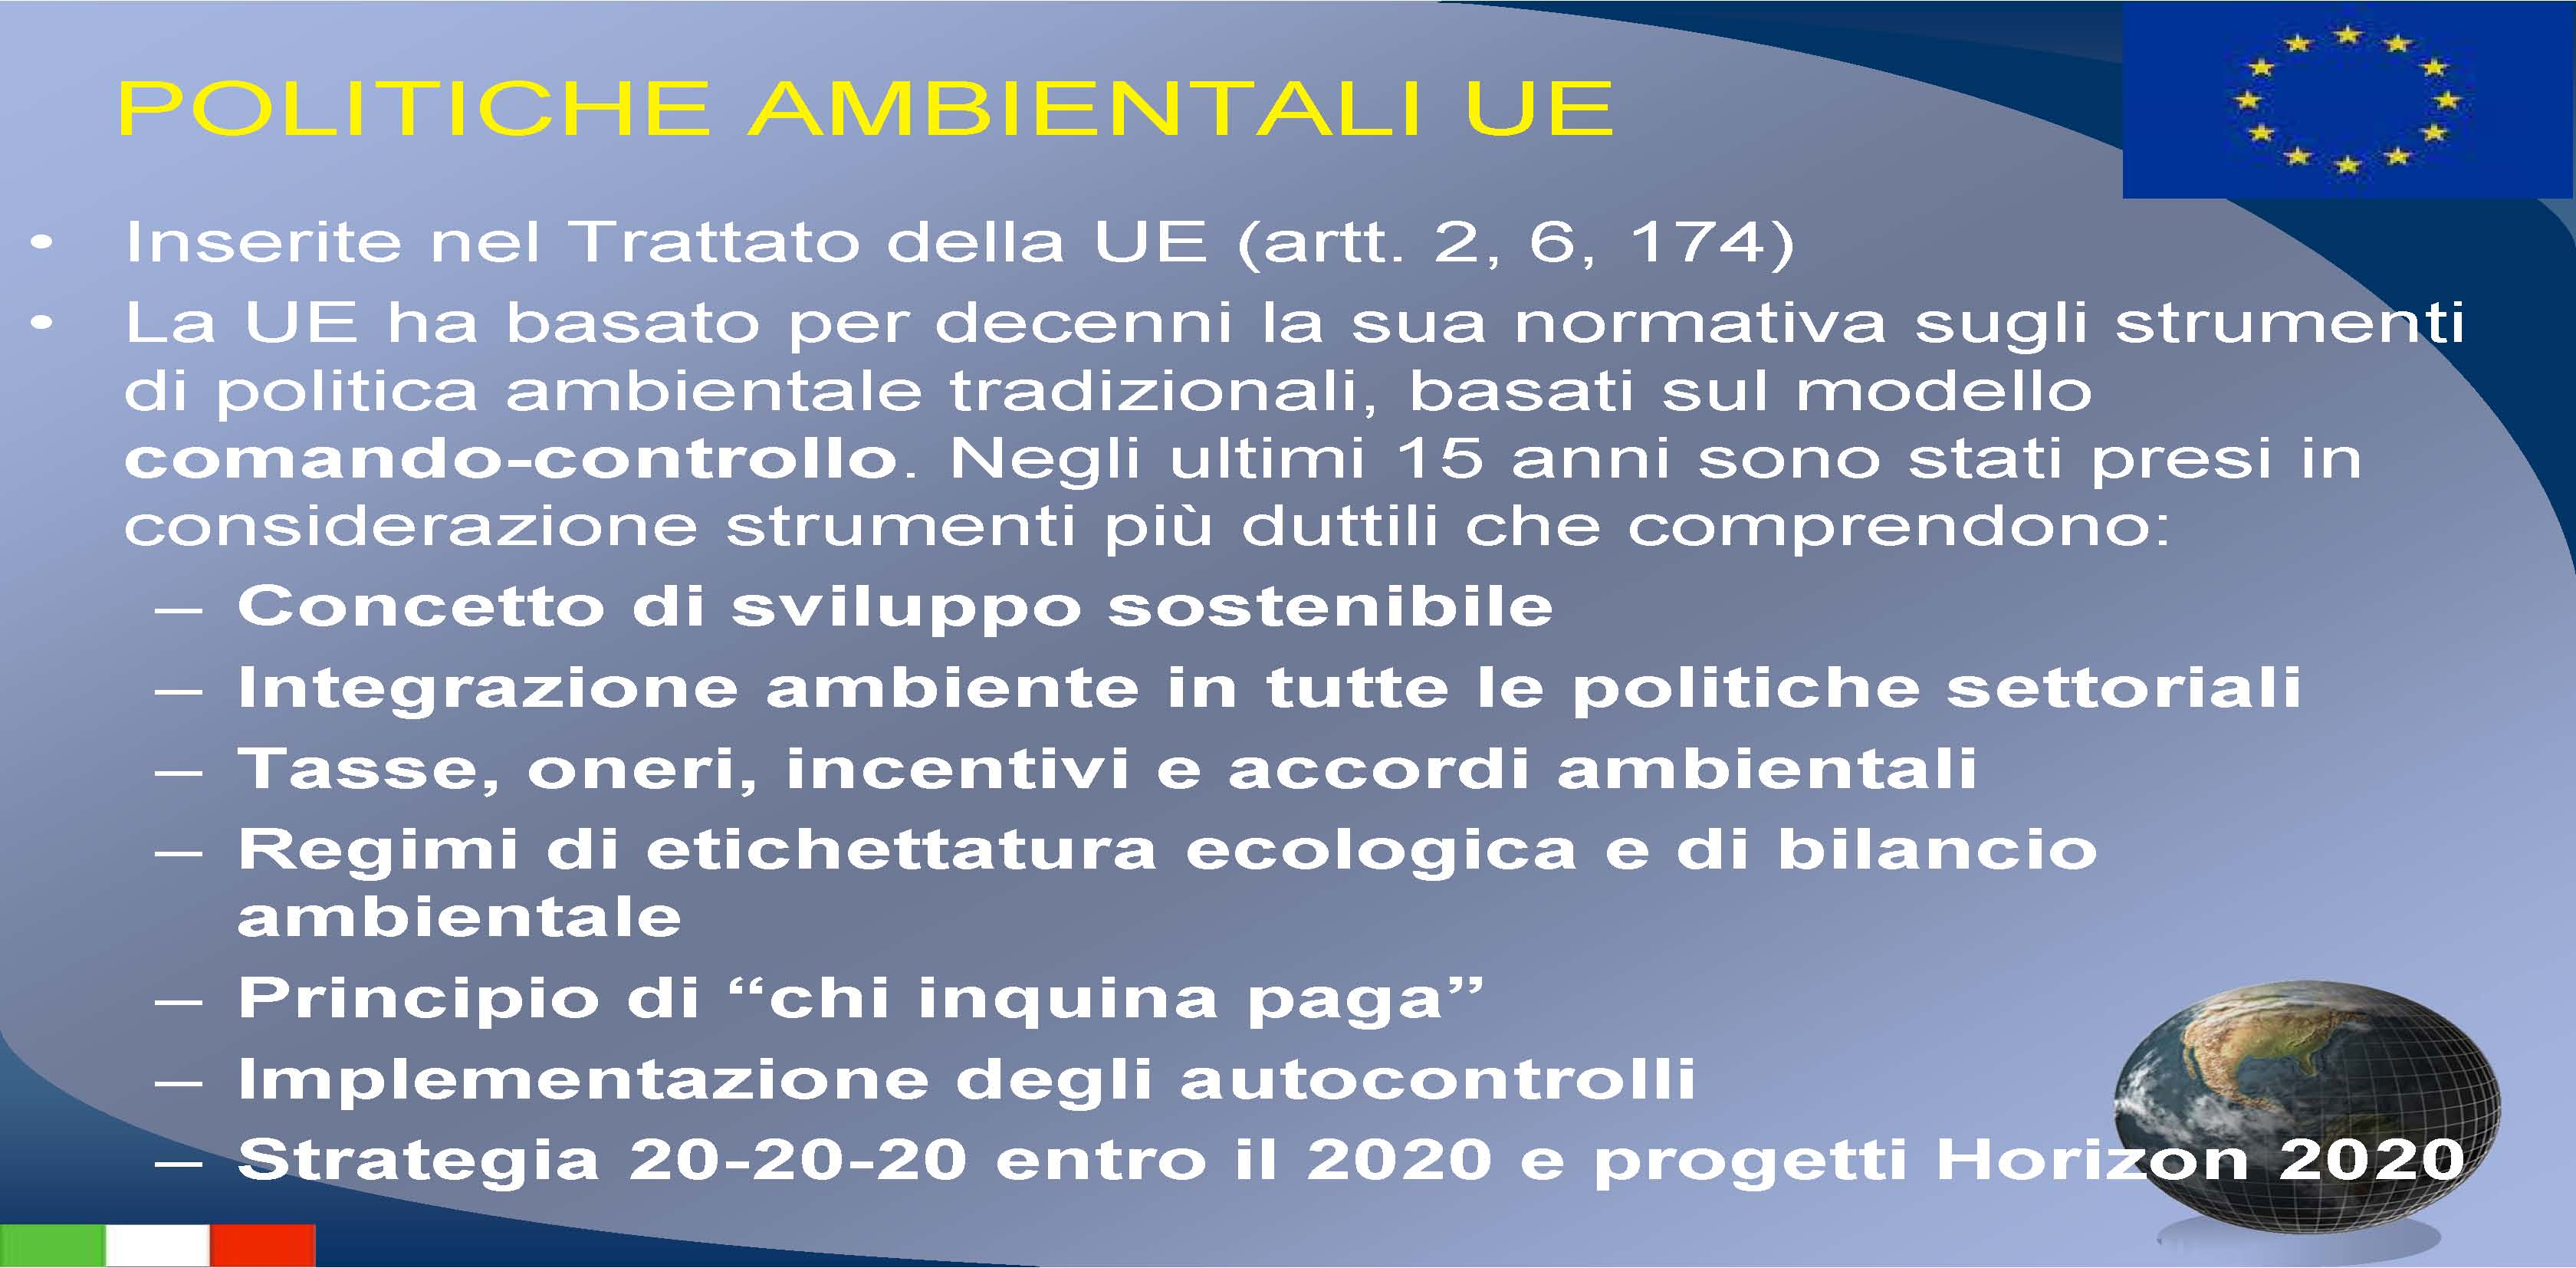
\includegraphics[width=0.7\textwidth]{22/image2.jpeg}
	\end{figure}

Le politiche ambientali italiane sono le politiche ambientali
dell'Unione Europea.

Pro: uniformità di legislazione.

Contro: se l'Italia non è abile a difendere le proprie ragioni a
Bruxelles, arrivano direttive molto difficili da rispettare (lo stato va
incontro a procedure d'infrazione).

Come vengono impostate le politiche ambientali?

\emph{Politiche principali}:

\begin{itemize}
\item
  sviluppo sostenibile
\item
  integrazione dell'ambiente in tutte le politiche settoriali
\item
  tassi, oneri, incentivi ( chi inquina paga!)
\item
  principio di implementazione agli autocontrolli: le politiche
  ambientali responsabilizzano molto le imprese. Importante è fare in
  modo che i soggetti potenziali inquinatori collaborino.
\end{itemize}

Principi principali.

\begin{itemize}
\item
  A. \emph{prevenire}
\item
  B. \emph{responsabilità}
\item
  C. \emph{precauzione}: essere molto prudenti. Quando c'è un principio
  di rischio scegliere delle soglie di sicurezza che azzerino o riducano
  al minimo il rischio che fattori ambientali provochino danni alla
  salute.
\end{itemize}

Alcuni inquinamenti ambientali, come l'inquinamento atmosferico, non è
possibile ridurli a zero. L'obiettivo delle politiche e delle leggi che
hanno recepito le direttive europee è quello di scendere ad un livello
tale per cui l'inquinamento abbia un effetto limitato secondo i principi
di precauzione. Questa soglia idealmente dovrebbe essere di 1 morto su 1
000 000/anno che può arrivare ad 1 morto su 100 000/anno, il prezzo che
paghiamo per non fermare il mondo. Questo perché non si può pensare di
vivere senza riscaldamento domestico, senza muoverci, senza determinate
attività che incidono sull'ambiente.

Questo principio di precauzione deve portarci a rischi talmente bassi da
poter essere tollerati e considerati accettabili.

L'ambiente tende a tollerare questo rischio con il principio di
precauzione, pensare di andare a zero è utopia.

L'OMS sottolinea come l'ambiente dev'essere armonico e pulito per
raggiungere il completo benessere fisico, mentale e sociale.

Le politiche ambientali oggi si battono molto sul risparmio energetico
dove possibile, energie rinnovabili, e sullo slogan delle città sane e
sostenibili (auto elettriche, mezzi non inquinanti, corsie ciclopedonali
in sicurezza \ldots{}).

Altri 3 settori:

\begin{itemize}
\item
  \emph{green economy}: tematica al risparmio energetico (settore che
  anche nel momento di crisi non ha avuto grande difficoltà). Pannelli
  fotovoltaici, mezzi ibridi\ldots{}la sensibilità alle tematiche del
  risparmio energetico è crescente.
\item
  Burocrazia: le piccole medie imprese lamentano lentezza per le
  pratiche burocratiche ambientali.
\item
  Elemento positivo: il cittadino medio, oggi, quando compra un immobile
  si pone il problema dell'\emph{edilizia sostenibile}, cioè la classe
  energetica dell'edificio e a questo da un valore economico (10 anni fa
  non era così!). Il cittadino risparmia, in termini di spreco
  energetico, e allo stesso tempo guadagna l'ambiente perché s'inquina
  meno.
\end{itemize}

\begin{figure}[!ht]
\centering
	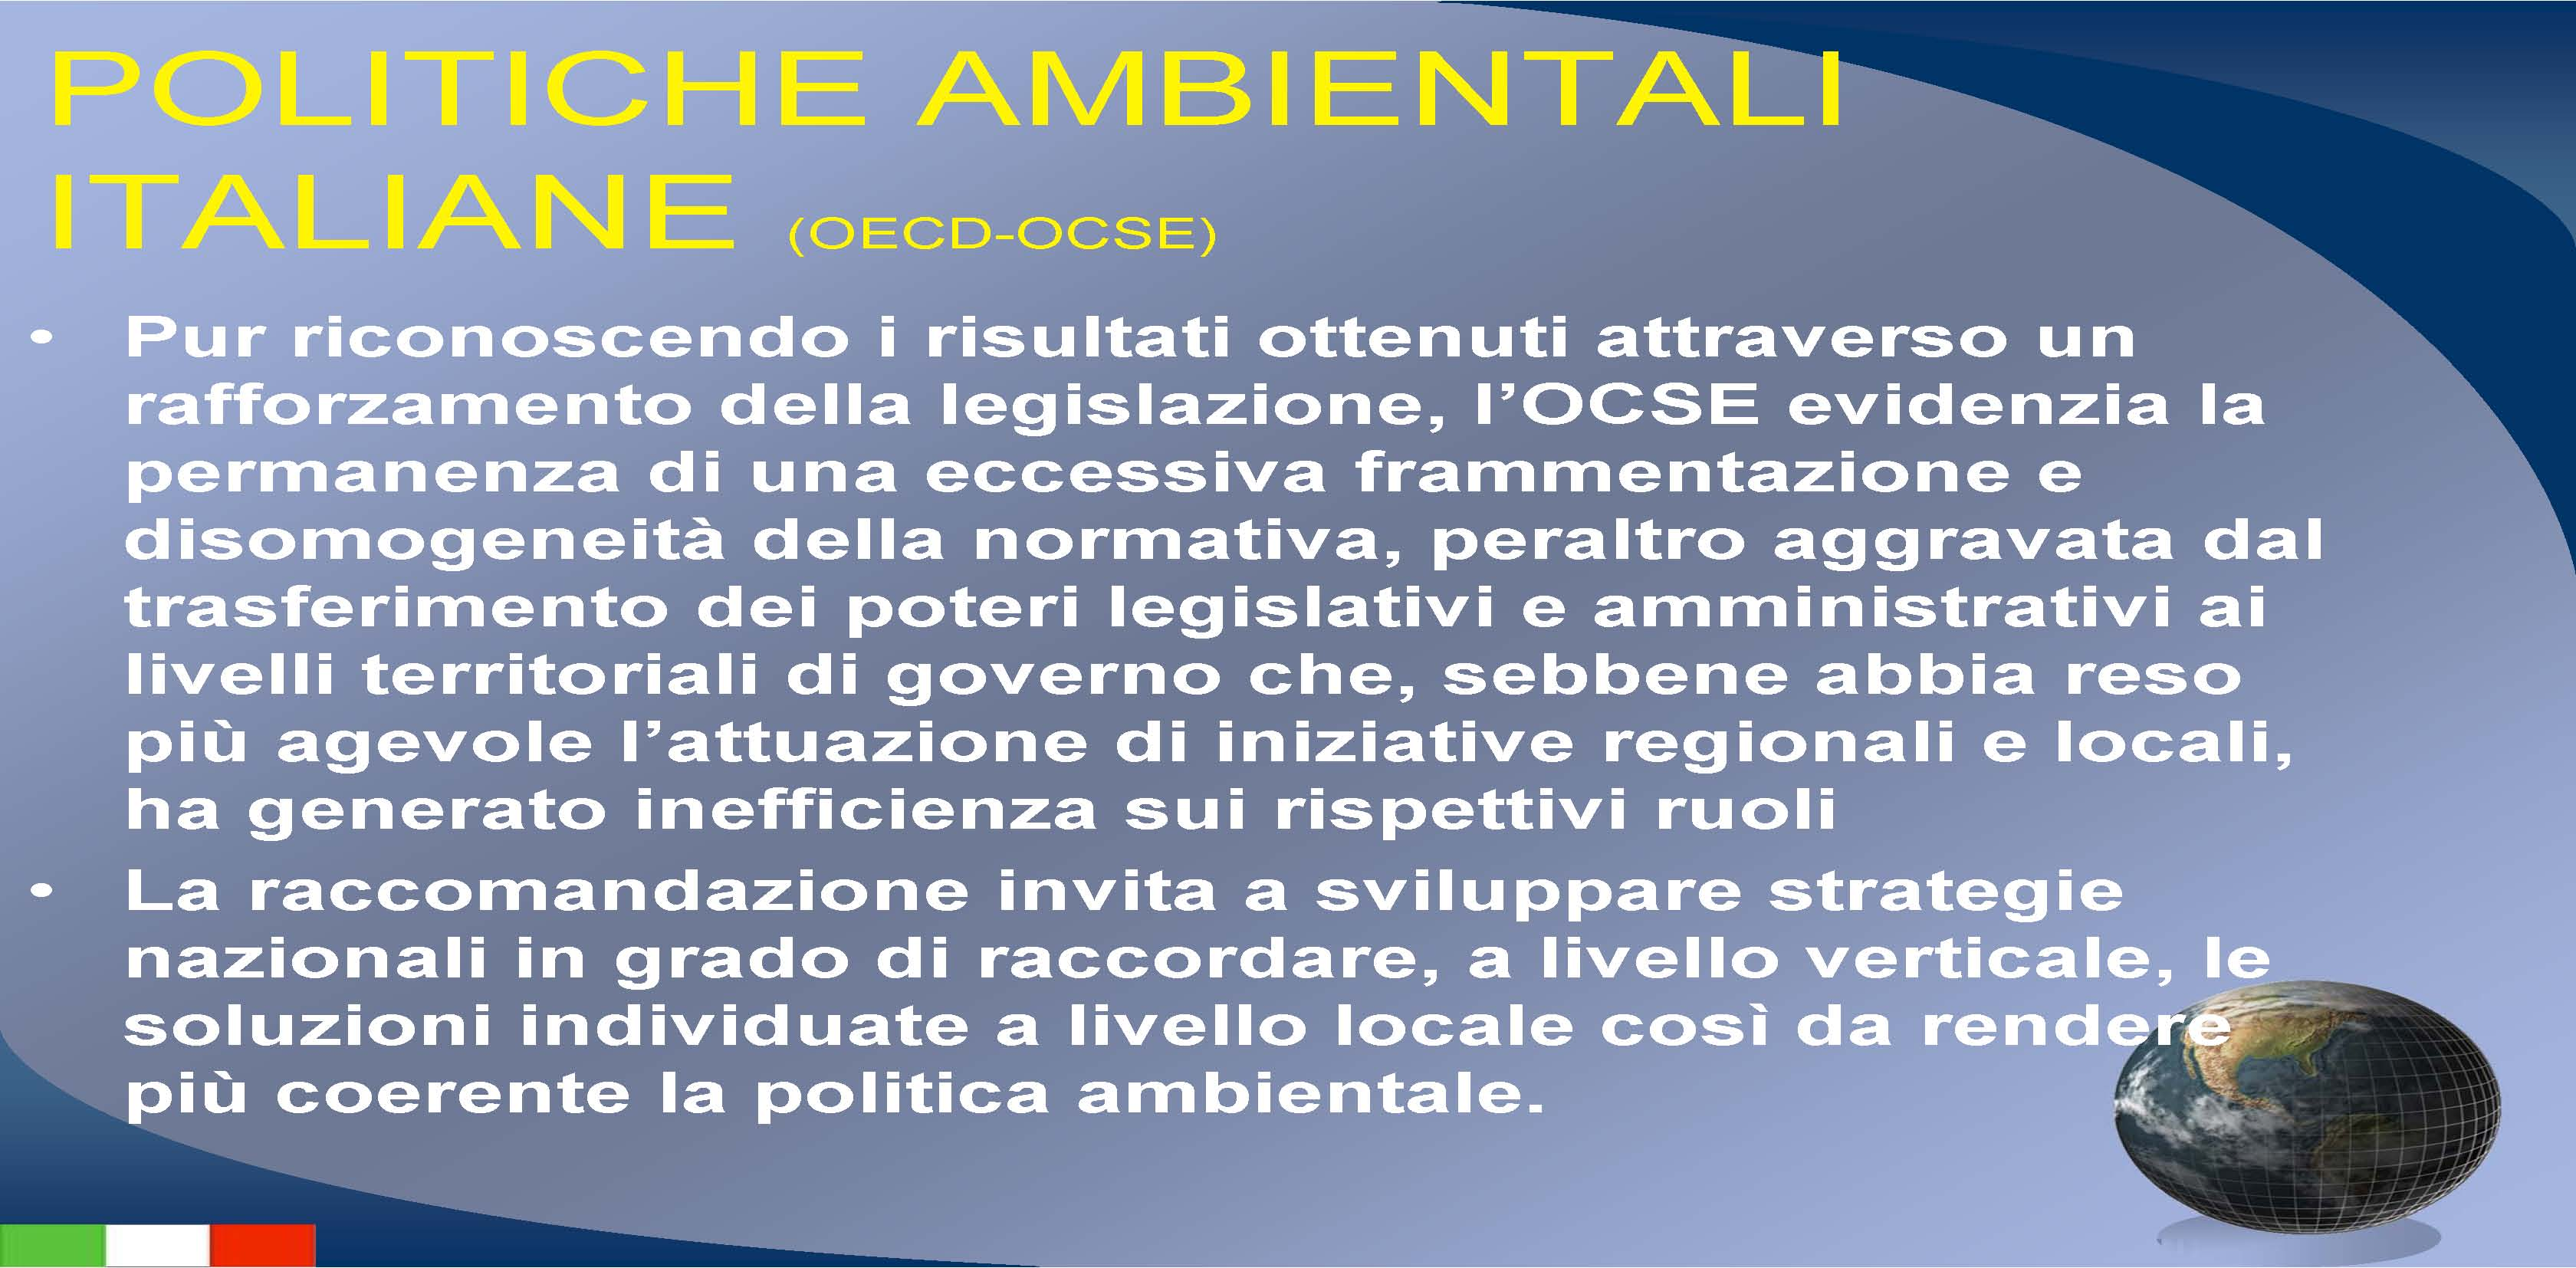
\includegraphics[width=0.7\textwidth]{22/image3.jpeg}
	\end{figure}

Cosa
dicono delle nostre politiche ambientali all'estero: RAPPORTI OCSE.

Si dice che la gestione delle politiche ambientali è non sempre efficace
e coerente. Non sempre i fondi pubblici sono spesi bene,
l'ecoinnovazione fatica a progredire.

Esiste in Italia un ``Codice dell'Ambiente'', dove sono unite tutte le
leggi e norme in unico corpo normativo (D.Lgs 152/2006). È un aspetto
positivo, un buon punto di partenza per una buona interpretazione a
vantaggio dell'ambiente.

Ci sono morti per inquinamento ambientale ma si deve fare attenzione ai
titoli dei
giornali.

\begin{figure}[!ht]
\centering
	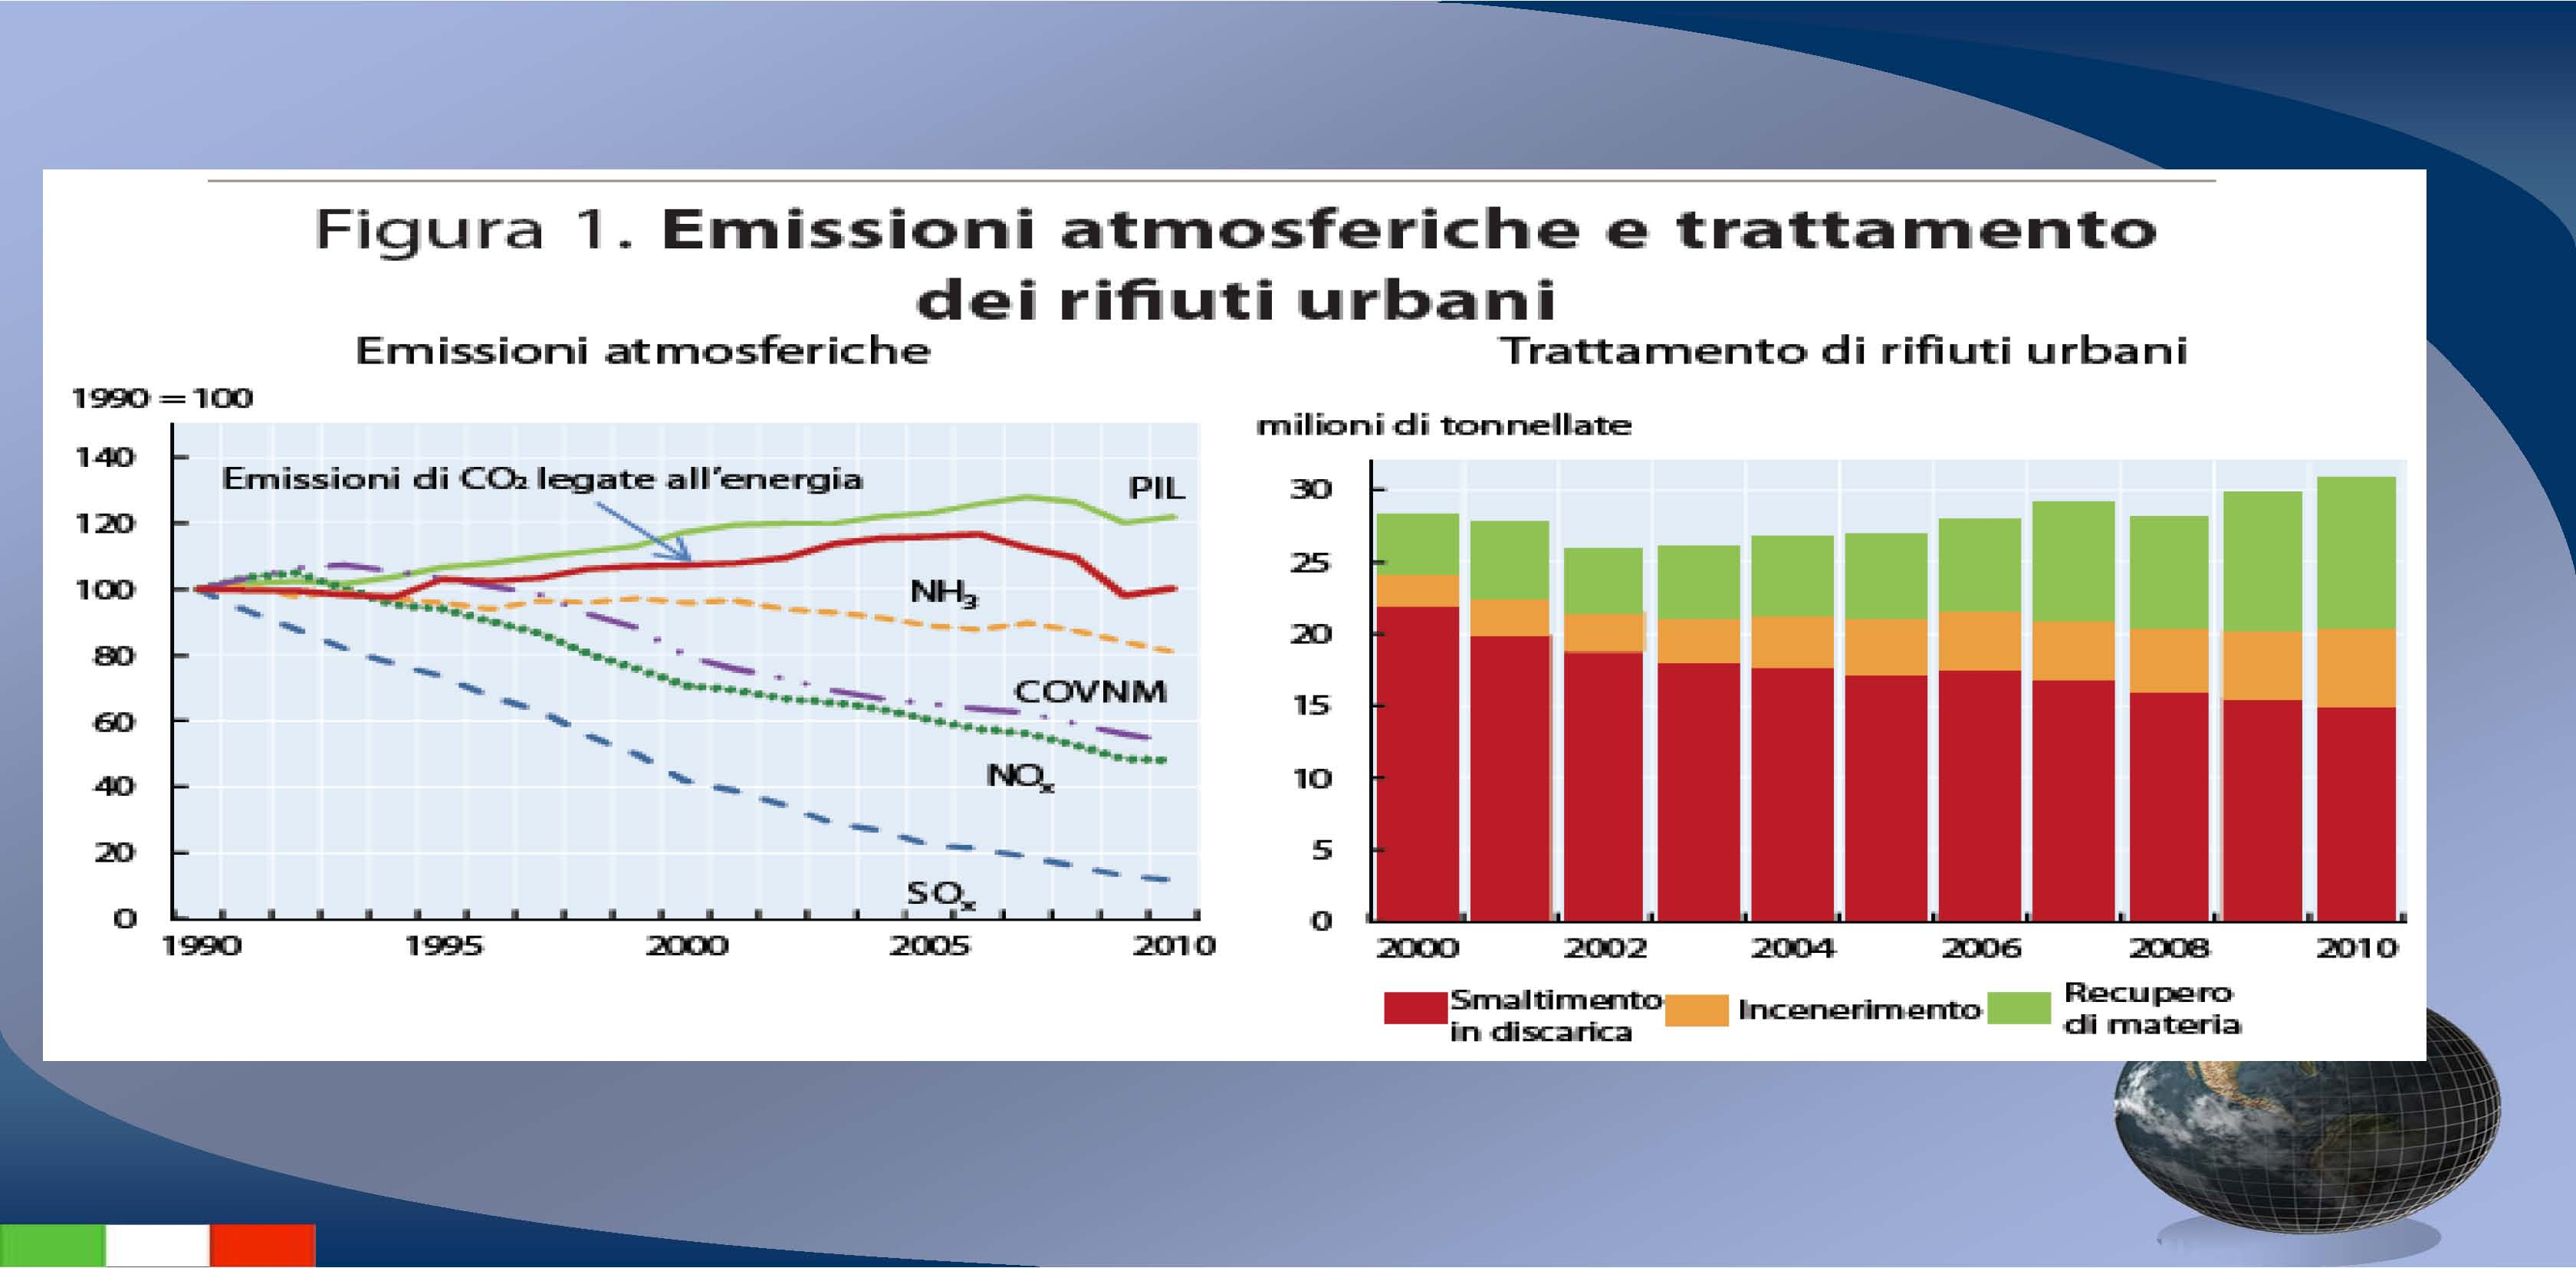
\includegraphics[width=0.7\textwidth]{22/image4.jpeg}
	\end{figure}

Il
grafico ci dice che dal 1990 al 2010 (in 20 anni) siamo riusciti a
ridurre sotto i livelli di pericolosità gli inquinamenti dell'aria da
inquinanti contenenti zolfo, composti contenenti azoto\ldots{} qualche
risultato nel 20ennio si è visto.

Flash rifiuti:

\begin{itemize}
\item
  in 10 anni non abbiamo implementato tanto la produzione dei rifiuti
\item
  raccolta differenziata implementata, non ancora a livelli ottimali.
\end{itemize}

Sono segnali positivi che portano ad una riduzione dello smaltimento in
discarica, meno consumi di suolo, meno inquinamento complessivo.

Finale del rapporto OCSE: sviluppare strategie nazionali più forti e
rendere più coerente la politica ambientale.

In italia ci sono circa 70 siti, di cui 20 critici, chiamati
``\emph{Siti di interesse nazionale per le bonifiche}''. Problema: negli
anni, aziende di vario genere hanno inquinato, hanno chiuso e se ne sono
andati lasciando il suolo inquinato. Mentre succedeva tutto ciò, la
legislazione era molto più morbida e meno restrittiva. Risultato
attuale: in Italia ci sono circa 50 siti ancora inquinati da bonificare
con costi molto alti.

Es: caso Terra dei fuochi, caso Ilva, emergenze rifiuti, incrementi di
malattie legate agli inquinamenti.

L'epidemiologia insegna che c'è un tempo di latenza tra l'esposizione ai
fattori di rischio e la malattia. Questo tempo negli inquinanti
ambientali è sempre molto lungo: quello che fotografiamo oggi, è ciò che
è stato dal punto di vista dell'inquinamento 20/30 anni fa! Le politiche
ambientali devono tenere conto di questi tempi di latenza molto lunghi,
quello che facciamo oggi di buono si vedrà, in termini di risparmi di
malattie laddove ci sono inquinamenti, in futuro.

IL ``tiro alla fune'' sulle politiche ambientali deriva da interessi
contrapposti. Da un lato la tutela dell'ambiente, restrittiva rigorosa,
rispetto delle norme comunitarie di solito molto stringerti. Dall'altro
lato le esigenze delle imprese, le così dette ``semplificazioni allo
sviluppo economico''. Le politiche ambientali \emph{vivono} con il tiro
alla fune, sono molto complesse e le esigenze in gioco molto forti.
Ideale sarebbe tutelare la salute senza compromettere lo sviluppo
economico, ma questo non sempre succede ed è fattibile.

Rapporto OCSE: politiche frammentarie ed estemporanee.

L'Italia per alcuni ambiti, come i pannelli fotovoltaici, ha utilizzato
leve economiche per spostare alcuni interessi e per far si che alcune
attività fossero favorite e diventassero ambite. È stato predisposto un
sistema all'incentivo di utilizzo di energie rinnovabili.

Il problema della manovra del pannello fotovoltaico è che la manovra è
stata fatta in modo talmente incentivante che gli scempi, in alcuni
casi, che ne sono venuti fuori, sono eclatanti. È un esempio di come la
politica ambientale è stata ben fatta, non si sono misurati gli
incentivi in relazione ai costi d'investimento, ed è stato ritenuto un
business talmente interessante che alcune aziende, anche estere, hanno
comprato interi campi ai contadini e hanno messo pannelli fotovoltaici
al posto delle coltivazioni. Quando lo stato si è accorto del problema
ha `messo una pezza', ma intanto si sono riempite di pannelli alcune
zone anche di pregio ambientale.

\begin{figure}[!ht]
\centering
	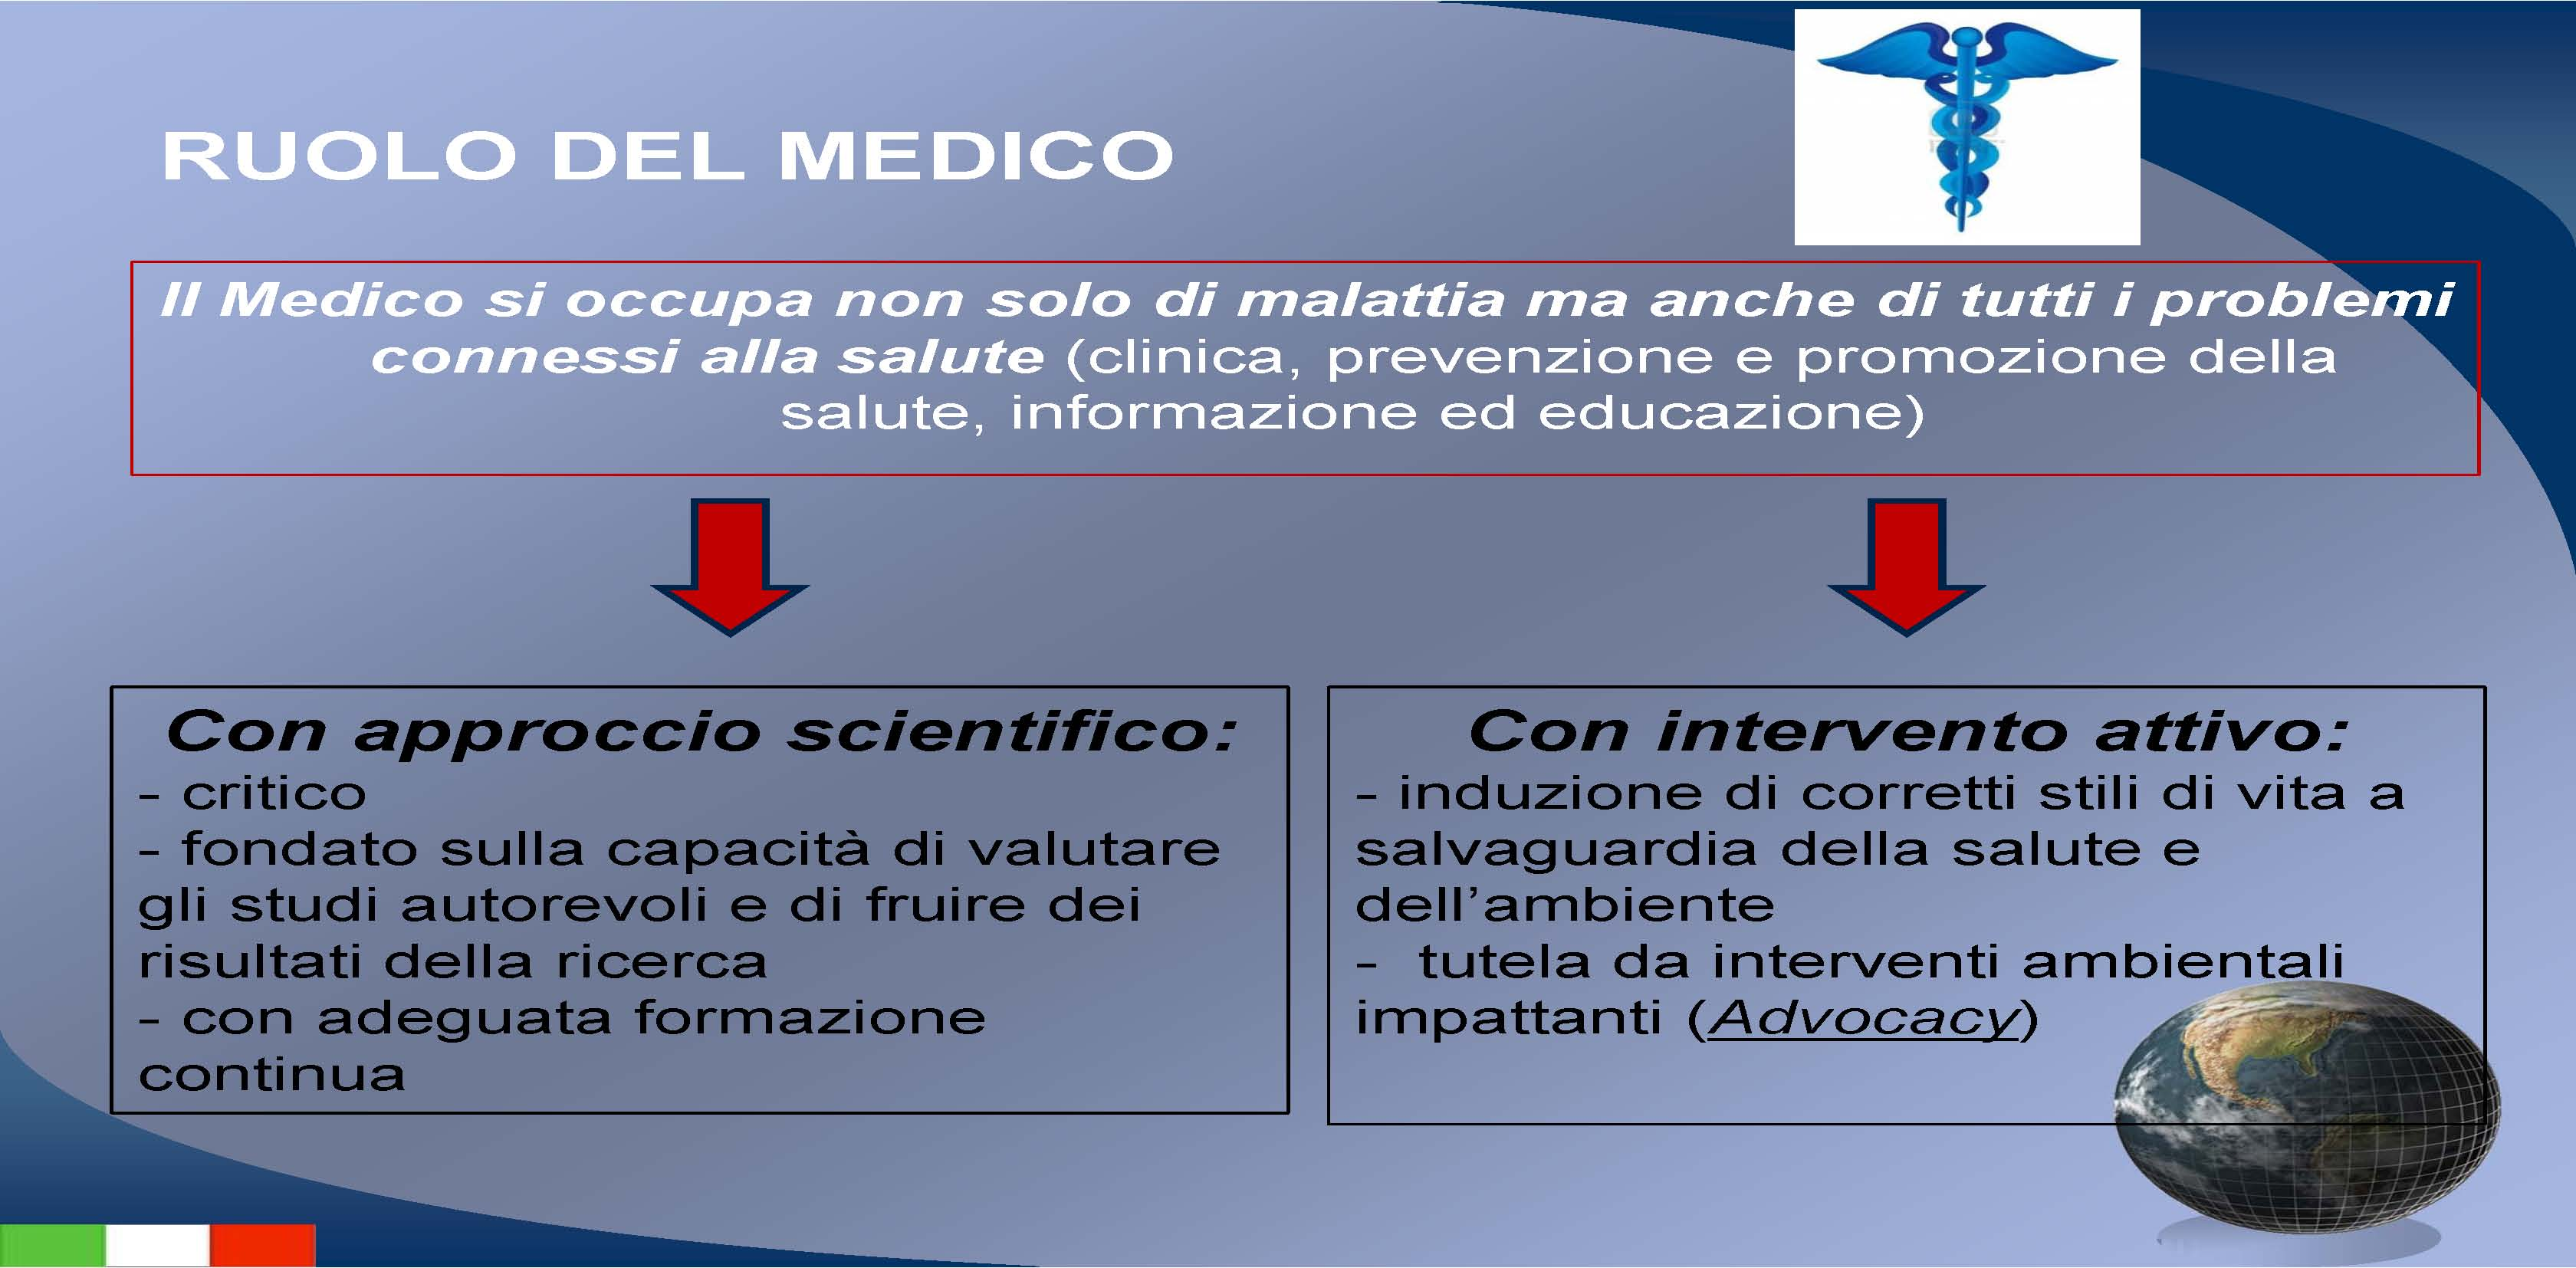
\includegraphics[width=0.7\textwidth]{22/image5.jpeg}
	\end{figure}

Ruolo del medico, in particolare medico di medicina generale perché ha
contatto con l'assistito, e svolge un ruolo importante in termini di
informazione.

Concetto cardine di tutte le politiche ambientali mondiali: definizione
di SVILUPPO SOSTENIBILE 1986 UN.

\textbf{\emph{Sviluppo Sostenibile}}: nuova alleanza tra uomo e natura
per operare una forma di sviluppo che permetta di soddisfare le esigenze
del presente senza compromettere le capacità delle generazioni future di
progredire e innovare le tecnologie.

Il problema dello sviluppo sostenibile è: come traduciamo questi
principi in politiche ambientali? Qui nascono i disaccordi\ldots{}

\begin{figure}[!ht]
\centering
	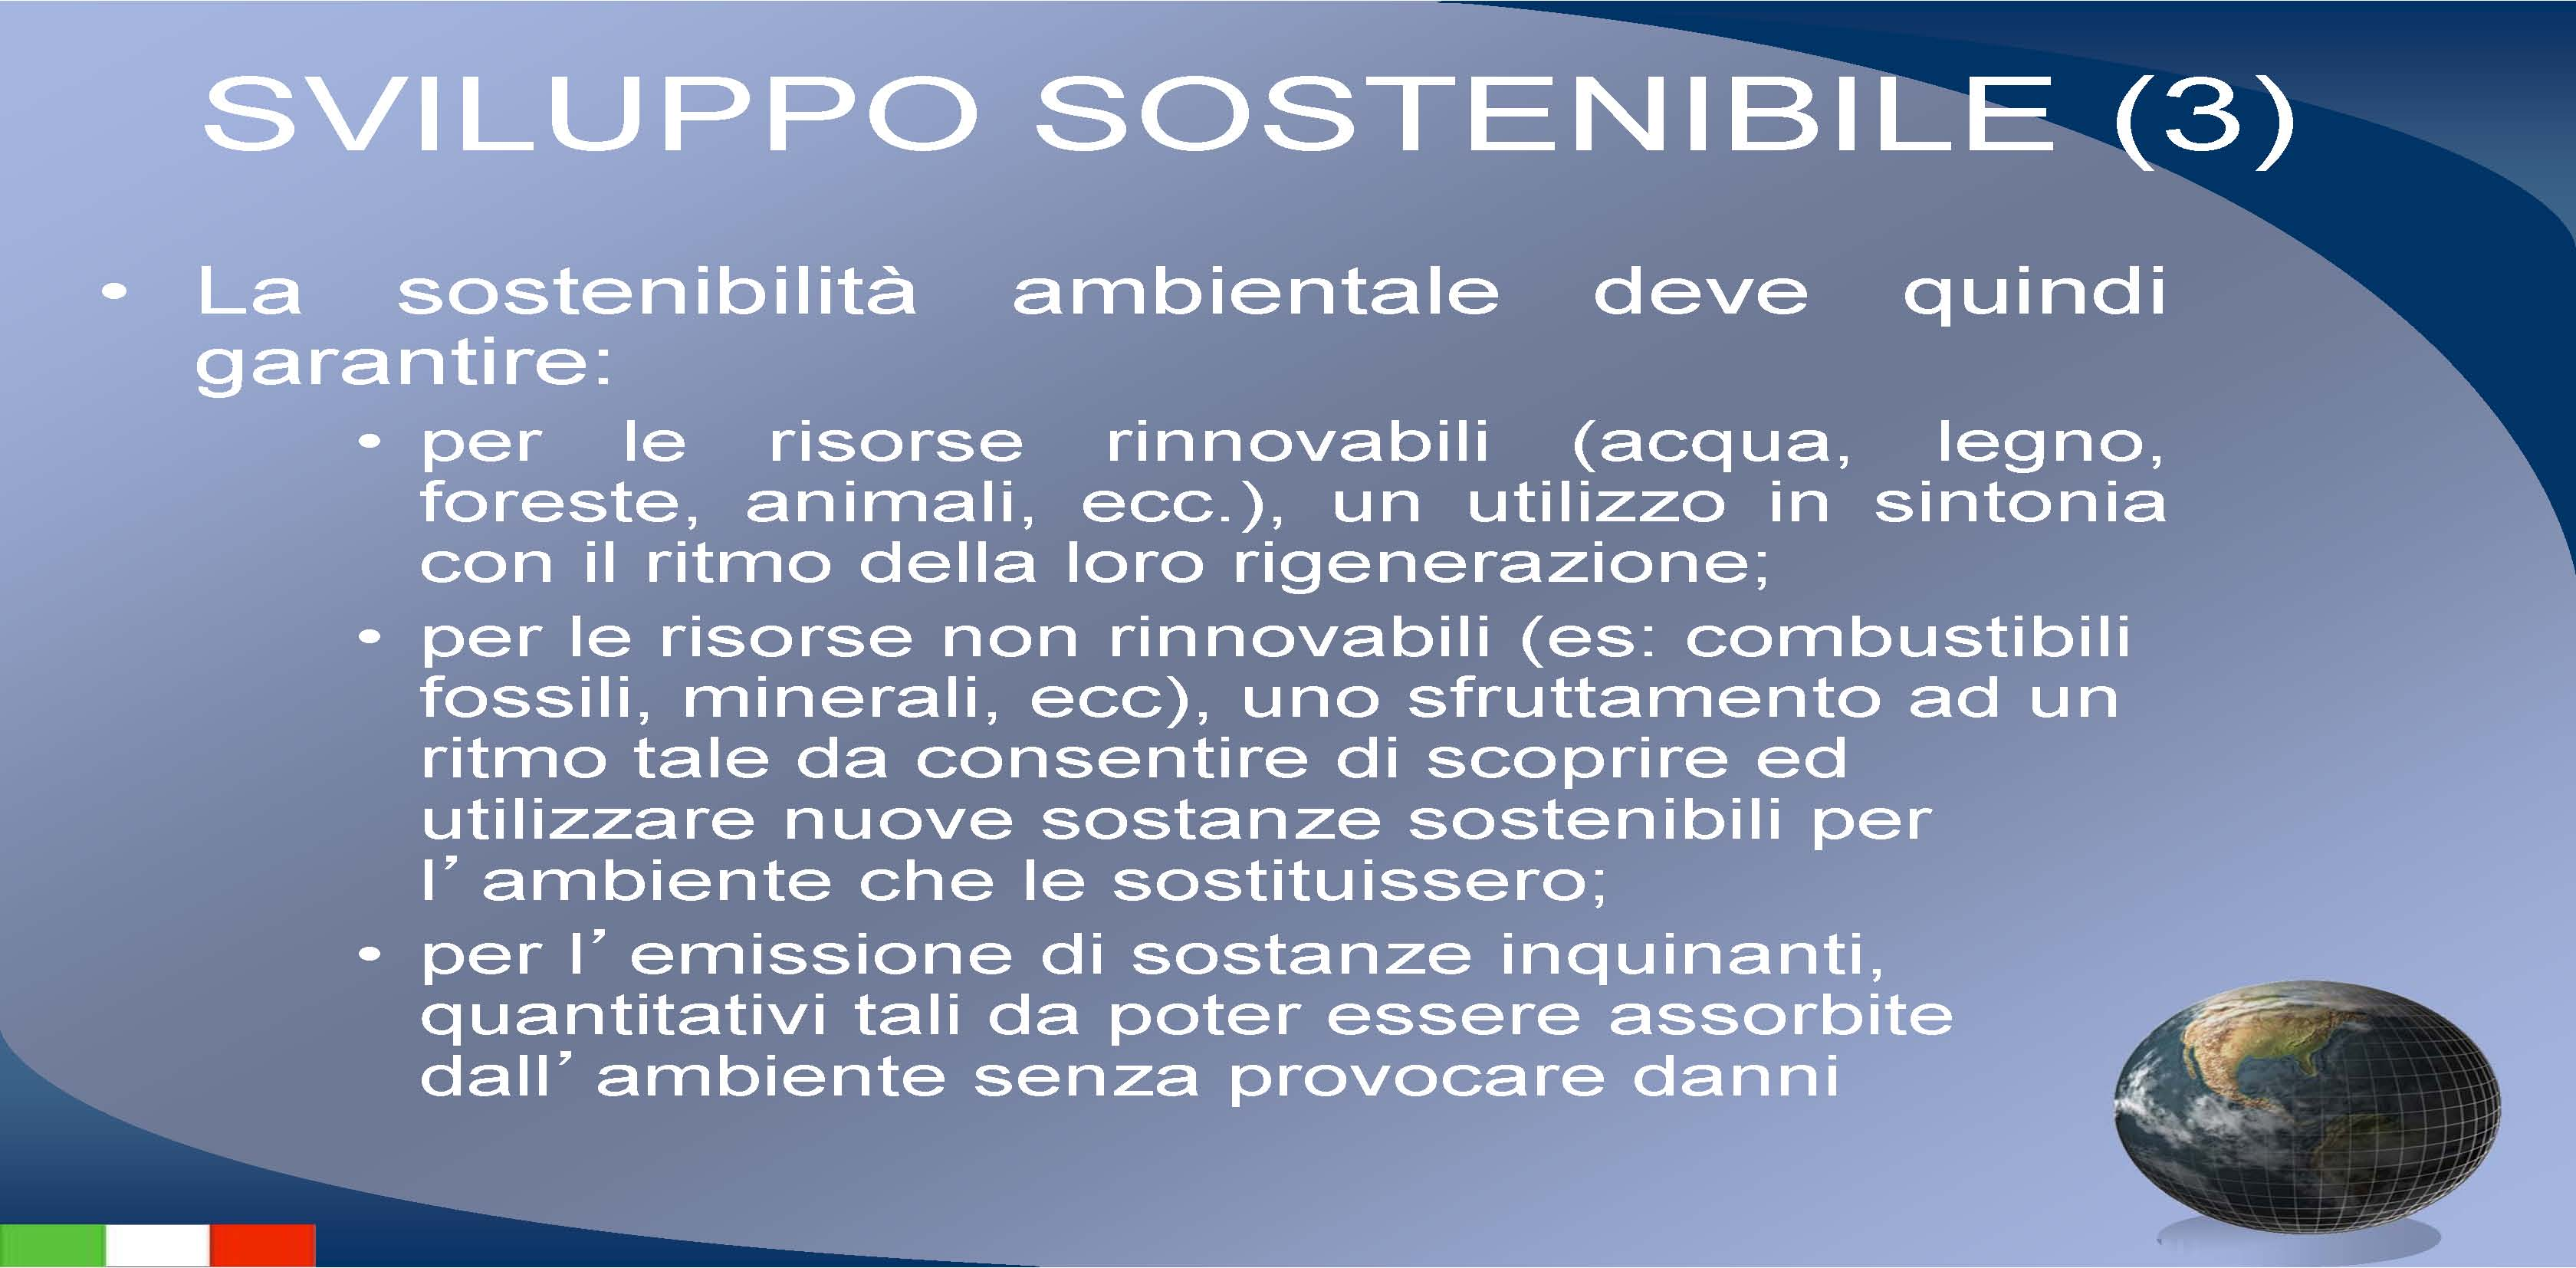
\includegraphics[width=0.7\textwidth]{22/image6.jpeg}
	\end{figure}
	
\textbf{Sindrome Nimby}: not in my backyard = non nel mio cortile!

Tutti approvano un nuovo `insediamento' però non vicino a casa propria.
La sindrome di Nimby è un atteggiamento che consiste nel ritenere
necessarie delle possibili opere ma contemporaneamente non nei luoghi
vicini.

Si trovano in Italia più di 354 contenziosi tra cui termovalorizzatori,
pale eoliche, discariche, inceneritori.

Es: le pale eoliche sono l'emblema dell'energia pulita. Anche queste
tutti le vogliono fare, ma nessuno vicino casa propria.

Risultato: abbiamo politiche ambientali molto rallentate da questi
fenomeni, che si riconoscono sotto il nome di Sindrome di Nimby.

\subsubsection{Rischio ambientale e determinanti di rischio}

\begin{figure}[!ht]
\centering
	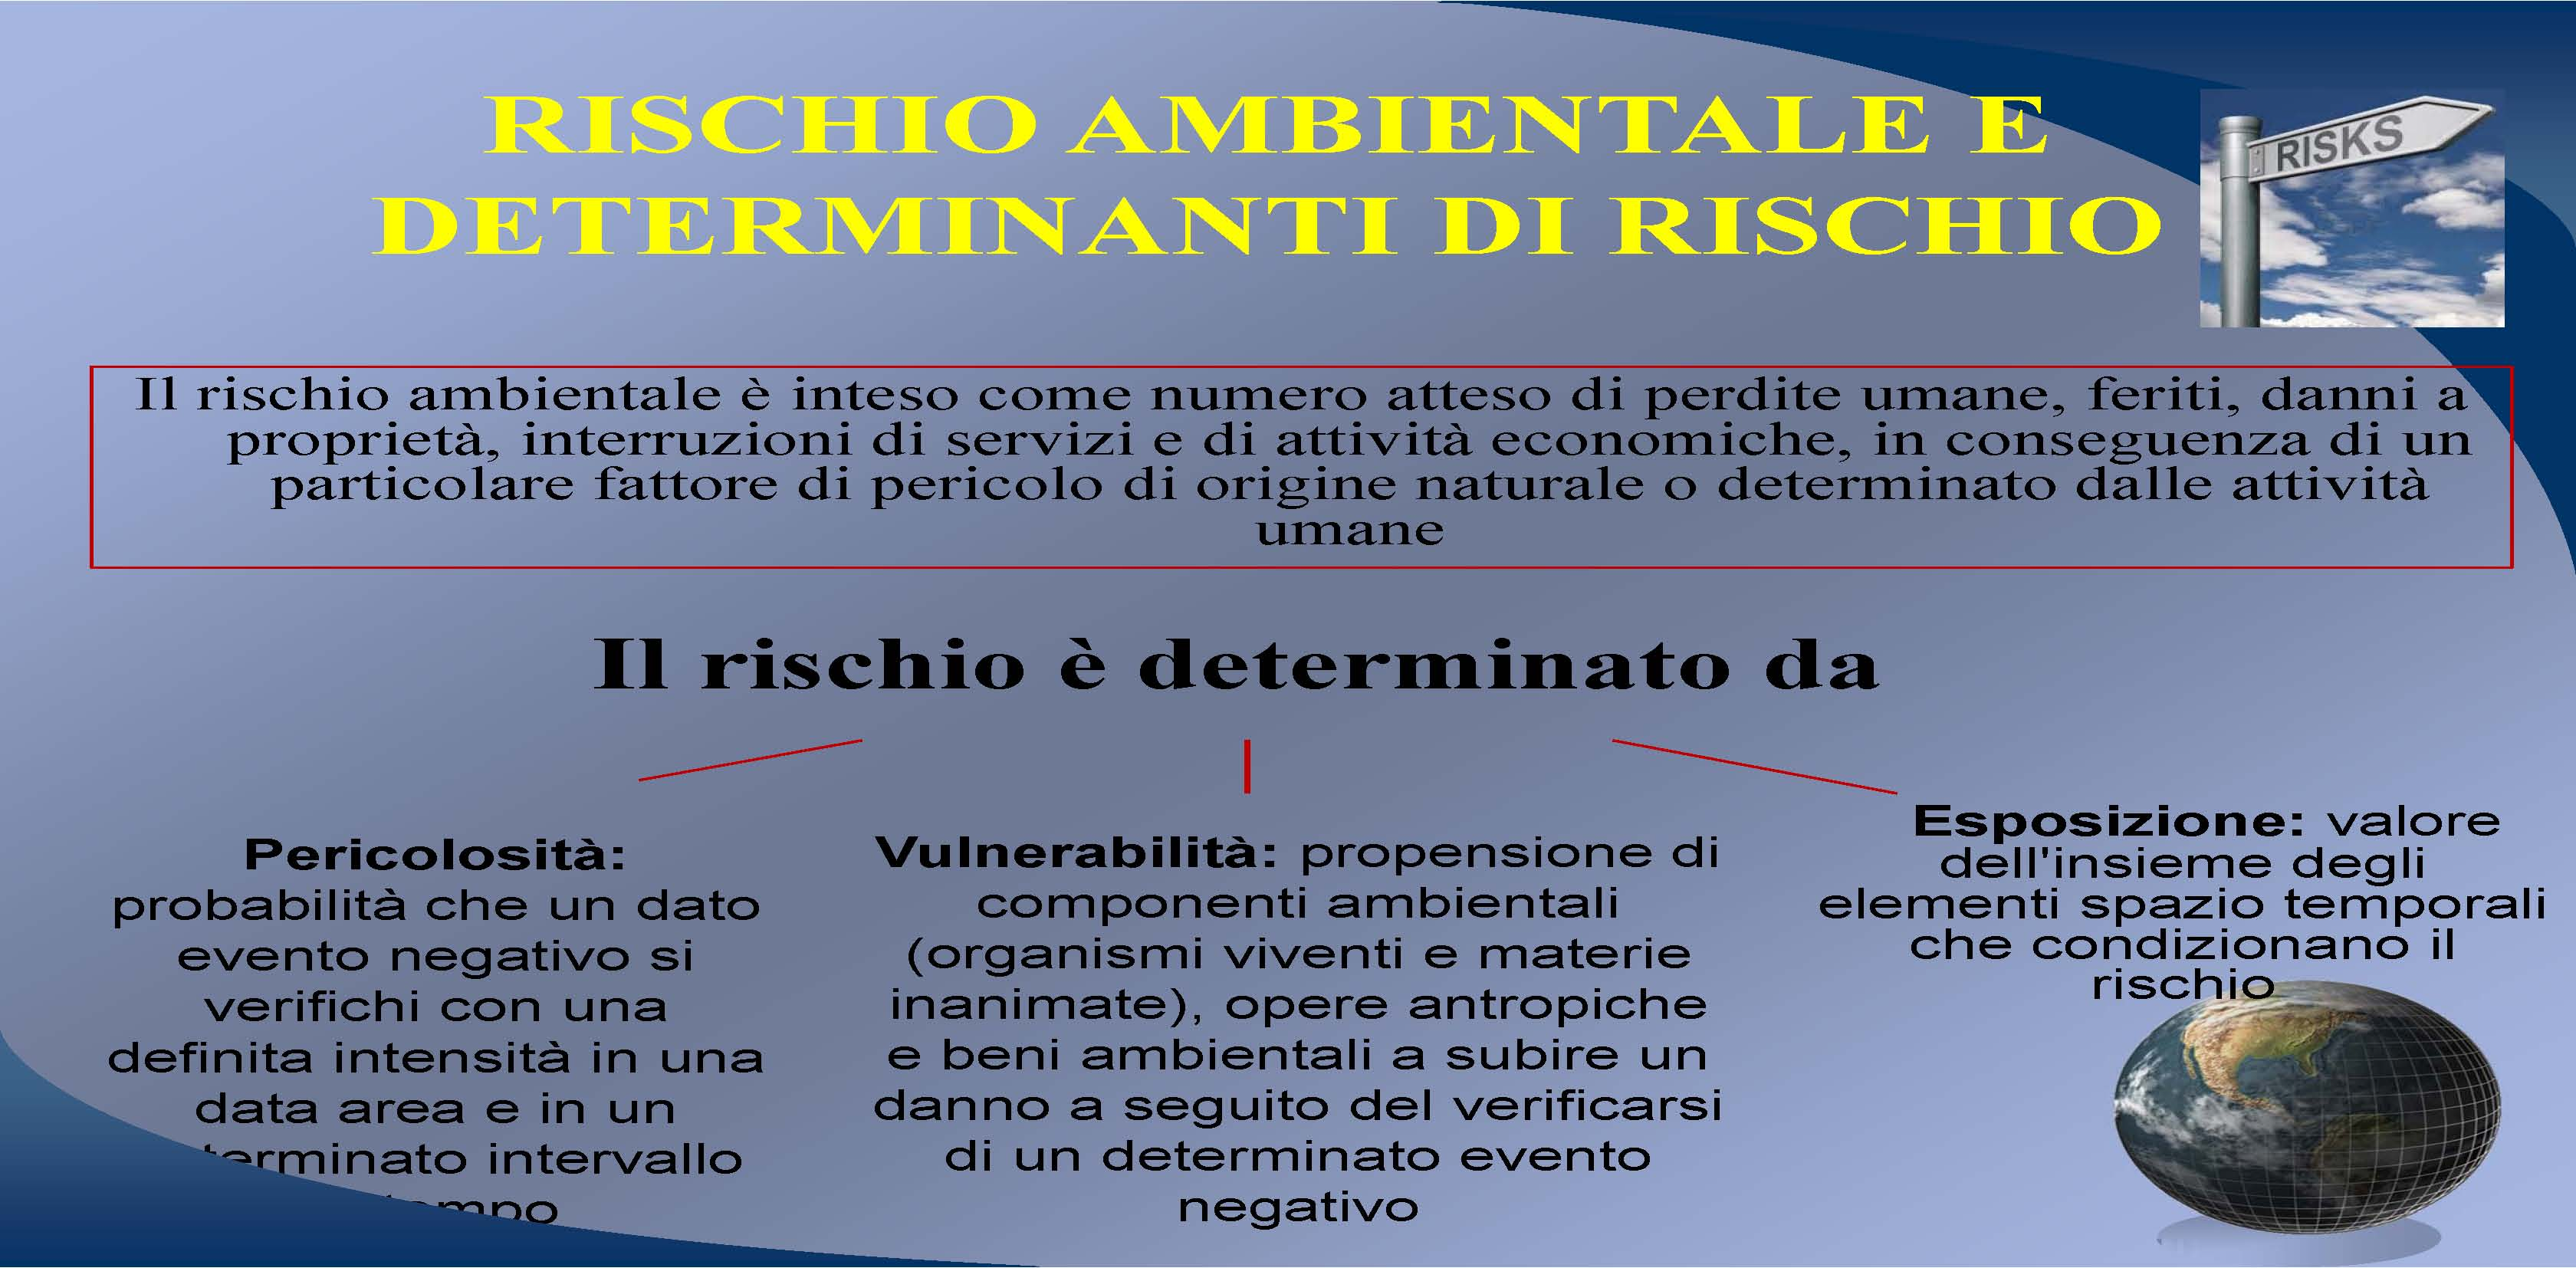
\includegraphics[width=0.7\textwidth]{22/image7.jpeg}
	\end{figure}
	
Ci sono 3 elementi che condizionano il \emph{\textbf{rischio
ambientale}} per la salute:

\begin{itemize}
\item
  \emph{pericolosità della sostanza;}
\item
  \emph{livelli di esposizione;}
\item
  \emph{vulnerabilità individuale.} Quando si vedono gli incrementi di
  mortalità nei giorni di alto inquinamento dell'aria (tipico nelle
  grandi città), muoiono i cardiopatici, i pz con malattie croniche, i
  grandi anziani.
\end{itemize}

Vivere in una grande città inquinata porta ad un rischio relativo di
mortalità rispetto alla campagna di 1,07: c'è un 7\% di mortalità in più
vivendo in città (rischio ambientale 1,07 da paragonare a valori 7/8 per
il fumo di sigaretta considerato rischio individuale).

Attenzione! Il 7\% in più non è spalmato per tutti allo stesso modo: i
fumatori ne risentono di più. La sinergia tra due fattori che agiscono
sullo stesso apparato crea un aumento del rischio (rischio legato alla
vulnerabilità del soggetto + il fumo di sigaretta).

Gestione del rischio cautelativa secondo il principio generale di
precauzione laddove è accettabile un rischio specifico di 1 morto su 1
000 000/anno, o comunque non più di 1 morto 100 000/anno, per qualunque
tipo di inquinamento ambientale. Qualunque tipo di insediamento che si
ritenga superi questa soglia accettabile non si fa.

Come gestiamo il rischio ambientale?

\begin{figure}[!ht]
\centering
	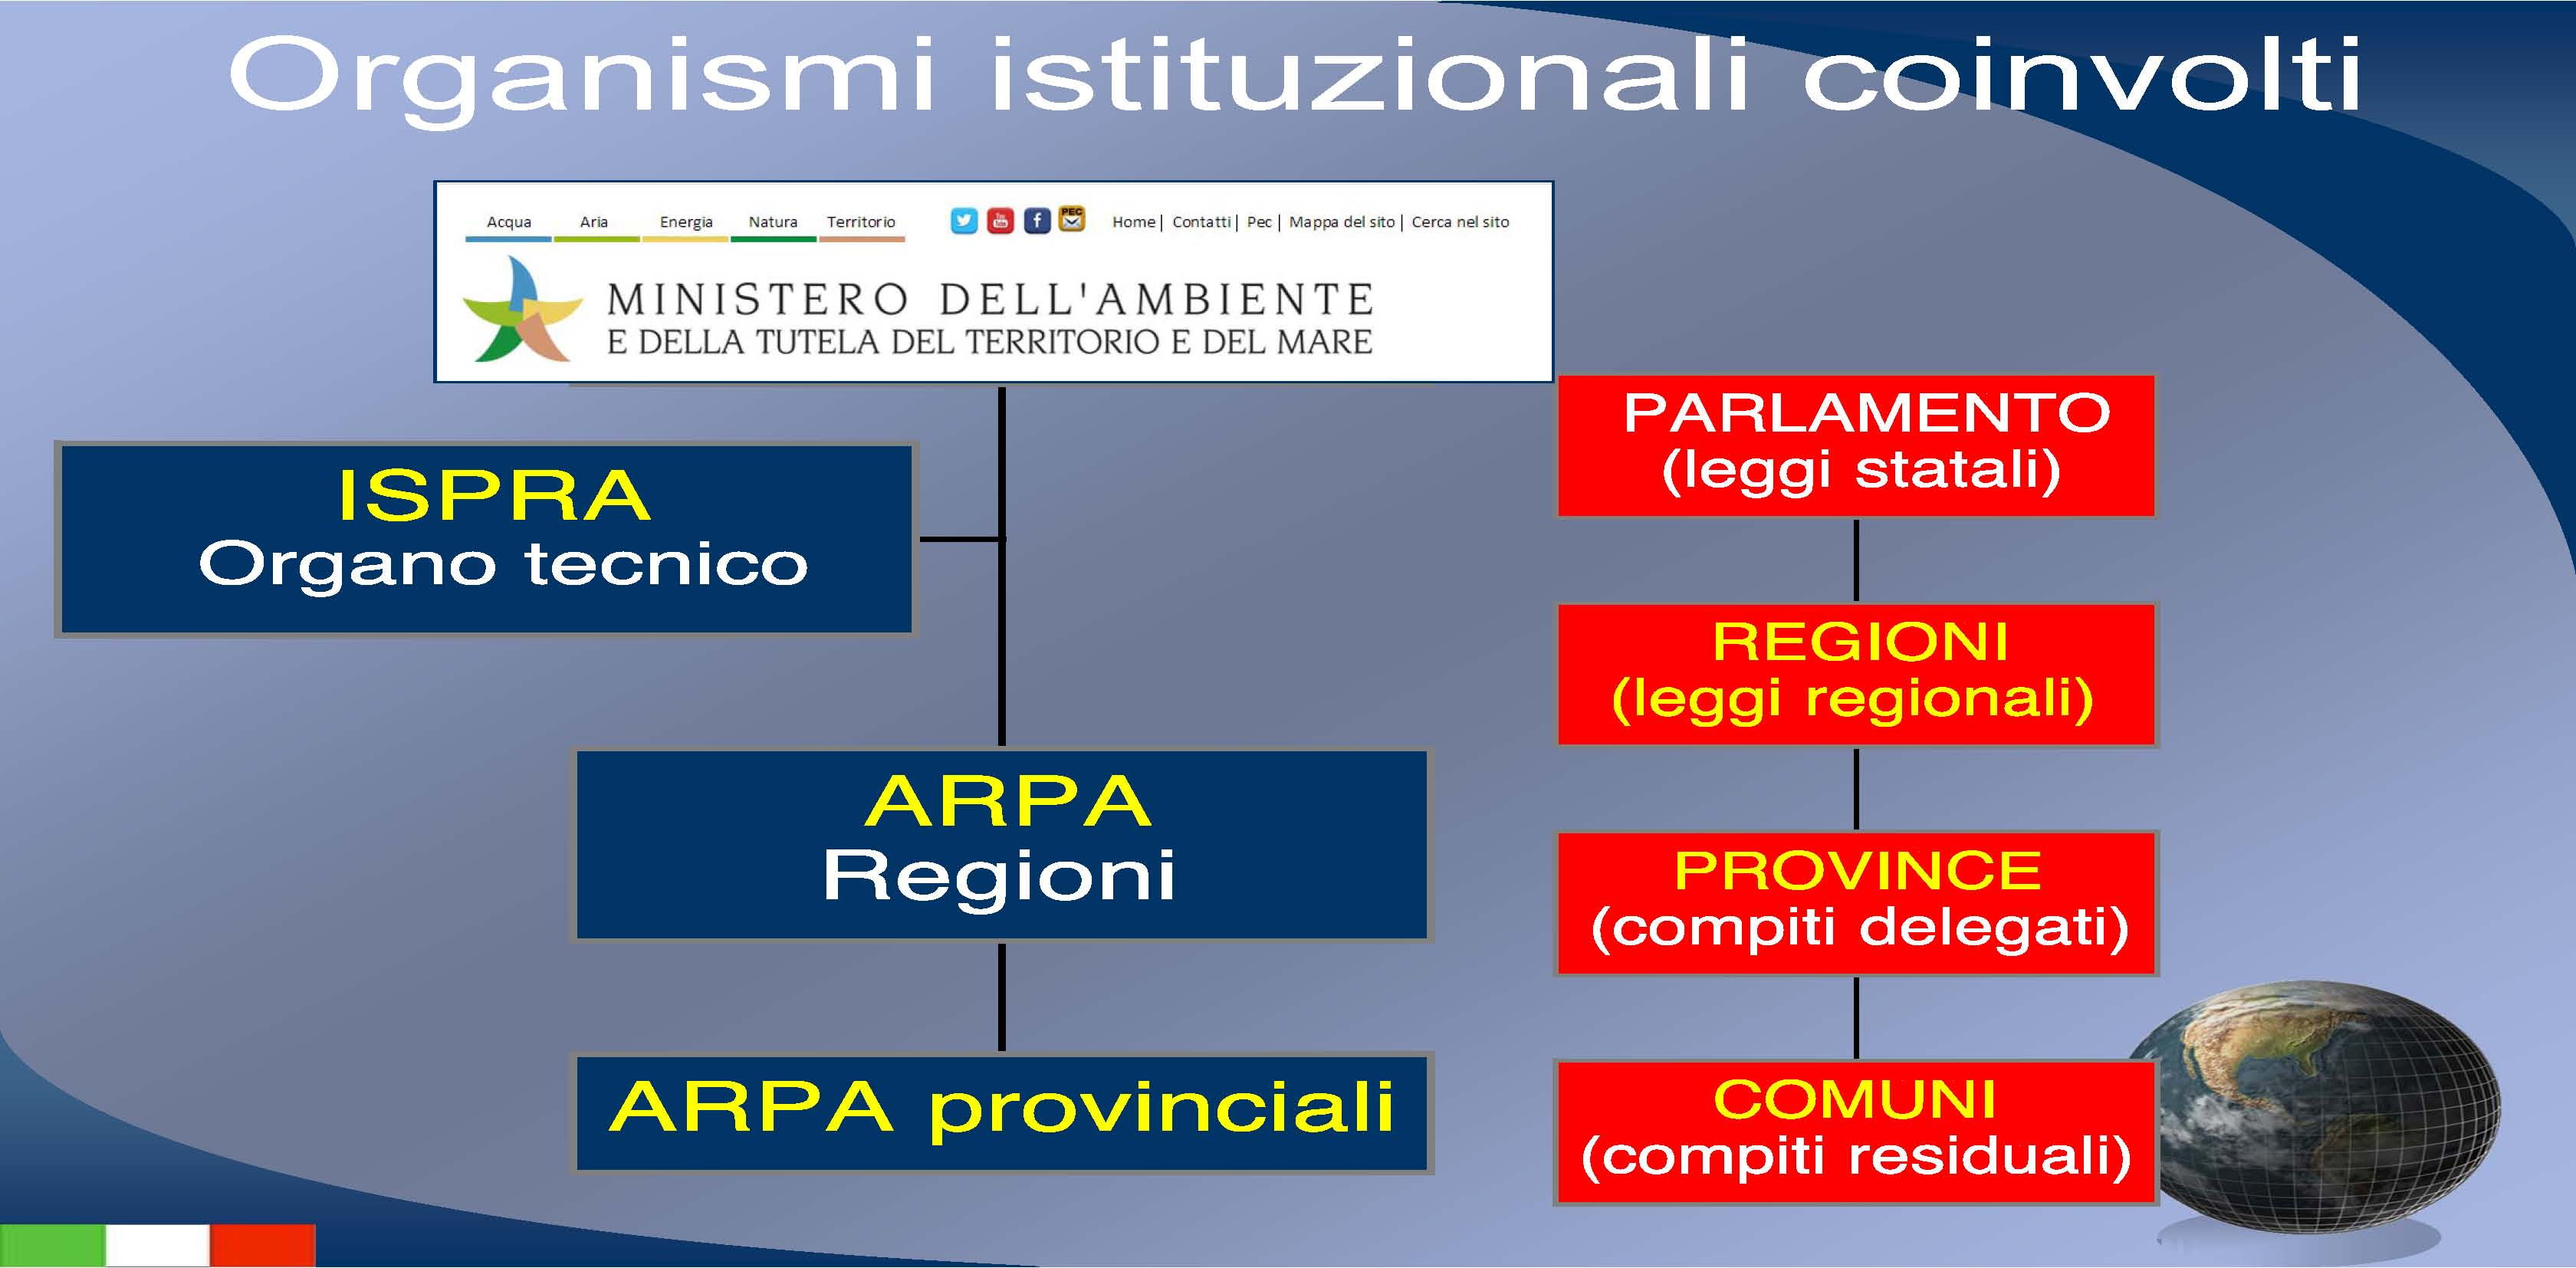
\includegraphics[width=0.7\textwidth]{22/image8.jpeg}
	\end{figure}
	
Si
gestisce identificando le misure idonee per eliminare o definire il
rischio accettabile con un monitoraggio sia ambientale che di parametri
biologici (se necessario) e con un'attività di comunicazione al rischio
ai cittadini che devono essere in grado di capire quali sono i rischi
(molte delle esposizioni sono legate ai comportamenti umani).

Il sistema dei controlli è gestito dalle ARPA: sistemi regionali per la
protezione ambientale, con articolazioni su base provinciale.

\subsubsection{Valutazione d'impatto ambientale}

I rischi ambientali, in generale, si prevengono a monte attraverso la
``\textbf{Valutazione di impatto ambientale}''. Oggi in tutta Europa
(dal '85) si valutano tutti i progetti in ordine alle ricadute negative
sull'ambiente e sulla salute in modo da arrivare ad ipotesi e sicurezze.

In particolare all'interno delle Valutazioni di Impatto Ambientale,
poniamo attenzione alla \textbf{VIS}, \textbf{Valutazione di Impatto
Sanitario}.

Es: costruzione della linea ferroviaria alta velocità Bologna-Milano
costruita vicina ad un'autostrada già presente. Si è pensato che fosse
meno rilevante da un punto di vista d'impatto ambientale. Nel caso della
linea ferroviaria, l'impatto ambientale comprende impatto visivo,
vibrazione, rumore.

In alcune casi, secondo le valutazioni d'impatto ambientale, sono
previste le \emph{mitigazioni}, delle soluzioni progettuali che riducono
l'impatto di certi fattori ambientali (es collinette o barriere per
attutire il rumore).

La \emph{valutazione impatto sulla salute} è una combinazione di
procedure metodi e strumenti con i quali si possono stimare effetti
potenziali sulla salute di una popolazione con proiezioni che danno
sufficienti garanzie per non fare o modificare alcuni insediamenti
considerati potenzialmente pericolosi per la salute umana.

Solo dopo aver fatto la valutazione impatto ambientale e la valutazione
impatto sanitaria si può arrivare alle autorizzazioni ambientali, parte
integrante delle politiche ambientali.

L'Autorizzazione Integrata Ambientale è un'autorizzazione rilasciata
dalla regione, provincia o comune (a seconda del tipo di insediamento)
che dovrebbe garantire il rispetto di tutte le norme.
